\chapter{Thermodynamica van elektrochemische cellen}\label{ch:b2:cell-thermodynamics}

Een waterstofbus met brandstofcellen draagt een stapel van een paar honderd dunne cellen. In elk ervan
combineren waterstof en de zuurstof van de lucht tot water zonder vlam, en de
energie komt eruit als een elektrische stroom. Twee getallen beheersen zo'n stapel, en
beide komen rechtstreeks uit tabellen van gibbsenergieën: geen enkele cel kan meer geven dan
\qty{1.23}{V}, en geen enkele brandstofcel, hoe volmaakt ook, zet alle energie van haar
waterstof om in elektrische arbeid. Dit hoofdstuk verbindt de spanning van een cel met
de \omterm{def:b2:reaction-free-energy:gibbs-energy}{gibbsenergie} van haar reactie, leidt de vergelijking van Nernst af die sinds het
deel van jaar~1 gebruikt wordt, en leest reactie-entropieën en reactie-enthalpieën af van een voltmeter
en een thermometer.

\begin{recall}
Het deel van jaar~1: cellen, halfcellen, anode en kathode, zoutbrug, celspanning,
elektrodepotentiaal, standaardpotentiaal en de standaardwaterstofelektrode,
de vergelijking van Nernst (daar aangenomen), evenwichtsconstanten uit
potentialen. \Cref{ch:b2:reaction-free-energy}: $\Delta_r G$, $\Delta_r G^\circ$
en $\Delta_r G = \Delta_r G^\circ + RT\ln Q$; het evolutiecriterium.
\Cref{ch:b2:chemical-potential}: activiteiten. Het schoolboek: elektrolyse.
\end{recall}

\begin{omfigure}
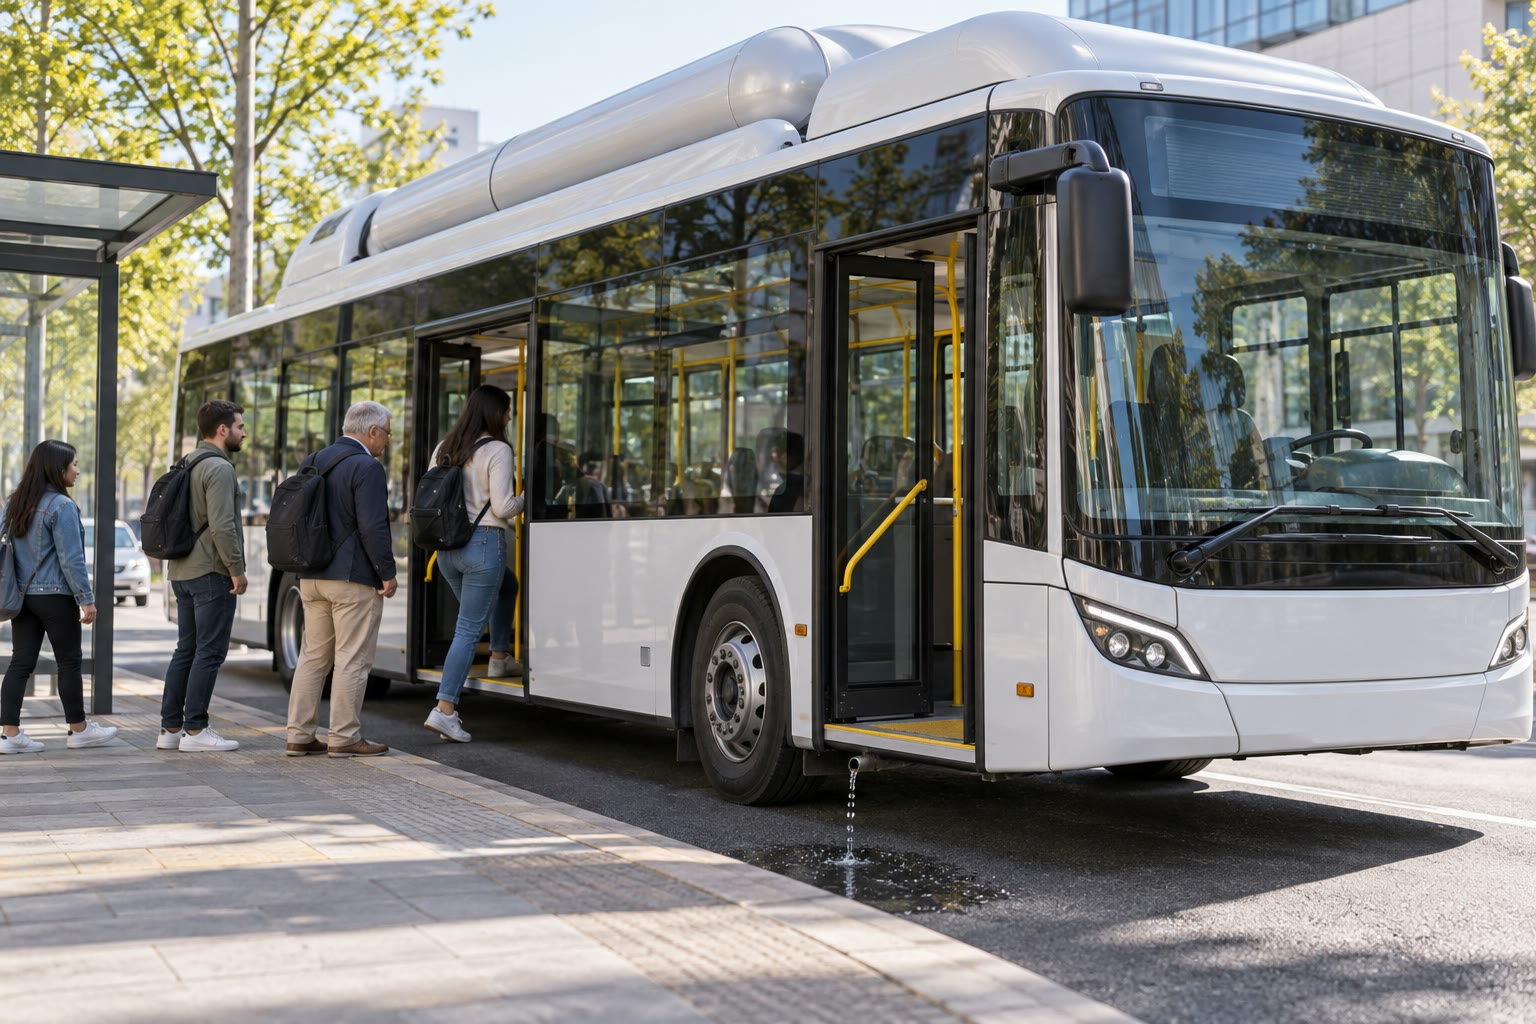
\includegraphics[width=0.62\linewidth]{images/book3/ai/b2-09-fuel-cell-bus.jpg}

{\small Een waterstofbus met brandstofcellen aan een halte: de waterstoftanks zitten onder de
bekleding op het dak, en de enige uitstoot is water, dat onder de bus drupt.}
\end{omfigure}

\section{Elektrische arbeid en de constante van Faraday}

\begin{definition}[Constante van Faraday]\label{def:b2:cell-thermodynamics:faraday}
De \emph{constante van Faraday}\index{constante van Faraday} is de elektrische lading van
één mol elementaire ladingen, $F = N_A e = \qty{96485.33}{C/mol}$.
% ledger: const:F
\end{definition}

\begin{proposition}[Doorgevoerde lading]\label{prop:b2:cell-thermodynamics:charge}
Als de reactie van een cel, geschreven met $n$ uitgewisselde elektronen, met
$\Delta\xi$ voortschrijdt, is de lading die door de uitwendige keten stroomt $Q =
nF\,\Delta\xi$.
\end{proposition}

\begin{proof}
Een voortgang $\Delta\xi$ brengt $n\,\Delta\xi$ mol elektronen van
de anode naar de kathode via de draad, elk met een lading $e$ in absolute waarde:
$Q = n\,\Delta\xi\,N_A e$.
\end{proof}

Wanneer een lading $Q$ door een spanning $U$ door een keten gedreven wordt, is de arbeid
die de keten ontvangt $QU$. Gezien vanuit de cel, die die arbeid levert, is
de elektrische arbeid die ze ontvangt $\delta W_{\text{el}} = -U\,\delta Q = -nFU\,
d\xi$.

\begin{omfigure}
\begin{tikzpicture}[font=\small, >={Stealth}]
  \draw[thick, rounded corners, fill=omDef!8] (0,0) rectangle (3.2,2.2);
  \node[align=center] at (1.6,1.1) {cel\\ (systeem)\\ reactie $d\xi$};
  \draw[->, thick, omThm] (3.2,1.6) -- (5.6,1.6) node[right, align=left] {$\delta W_{\text{el}}$ geleverd\\ $= nFU\,d\xi$};
  \draw[->, thick, omDef] (5.6,0.6) -- (3.2,0.6) node[pos=0, right, align=left] {$\delta Q_{\text{warmte}}$ ontvangen\\ (beide tekens mogelijk)};
  \draw[<->, thick] (1.6,2.2) -- (1.6,3.0) node[above] {omgeving bij $T$, $p$};
\end{tikzpicture}

{\small Een cel als thermodynamisch systeem bij constante temperatuur en druk:
ze wisselt warmte uit met haar omgeving en levert elektrische arbeid via
de uitwendige keten. Met de tekenafspraak van de eerste hoofdwet (ontvangen arbeid en warmte
positief geteld) is $\delta W_{\text{el}} = -nFU\,d\xi$.}
\end{omfigure}

\section{De gibbsenergie van een celreactie}

\begin{theorem}[Elektrische arbeid en gibbsenergie]\label{thm:b2:cell-thermodynamics:delta-g-nfe}
Een cel die bij constante $T$ en $p$ werkt, levert een elektrische arbeid die hoogstens
gelijk is aan de afname van haar \omterm{def:b2:reaction-free-energy:gibbs-energy}{gibbsenergie}: voor een voortgang $d\xi$ is
$nFU\,d\xi \leq -\Delta_r G\,d\xi$. Wanneer ze reversibel werkt (een oneindig
kleine stroom), geldt de gelijkheid, en is de celspanning de
elektromotorische kracht
\[
  \Delta_r G = -nFE .
\]
\end{theorem}

\begin{proof}
Eerste hoofdwet bij constante druk, met de volumearbeid apart:
$dH = \delta Q + \delta W_{\text{el}}$. Tweede hoofdwet: $dS \geq \delta Q/T$. Bij
constante $T$ en $p$ is $dG = dH - T\,dS \leq \delta W_{\text{el}} = -nFU\,d\xi$.
Met $dG = \Delta_r G\,d\xi$ is $\Delta_r G\,d\xi \leq -nFU\,d\xi$, dus
$nFU\,d\xi \leq -\Delta_r G\,d\xi$. Voor een reversibele verandering is de ongelijkheid
van de tweede hoofdwet een gelijkheid, en de spanning die dan gemeten wordt, zonder
stroom, is $E$: $\Delta_r G = -nFE$.
\end{proof}

Een cel kan dus alleen voorwaarts werken ($d\xi > 0$, arbeid leverend) als $\Delta_r G <
0$, dus $E > 0$ met de polen zo gekozen dat de geschreven reactie verloopt
van anode naar kathode. Een echte cel, waardoor een stroom loopt, levert
minder arbeid dan $-\Delta_r G$: het verschil wordt als warmte gedissipeerd in haar
weerstand en aan haar elektroden (\cref{ch:b2:current-potential-curves}).

\begin{example}[De daniellcel]\label{ex:b2:cell-thermodynamics:daniell}
Voor \ce{Zn + Cu^2+ -> Zn^2+ + Cu} is $\Delta_r G^\circ = \Delta_f G^\circ(\ce{Zn^2+}) -
\Delta_f G^\circ(\ce{Cu^2+}) = -147.06 - 65.49 = \qty{-212.55}{kJ/mol}$, en $n = 2$:
$E^\circ = 212\,550/(2 \times 96\,485) = \qty{1.10}{V}$, de spanning die gemeten wordt op een
daniellcel onder standaardomstandigheden.
% ledger: dfg:Zn2+_ao, dfg:Cu2+_ao, const:F, emf:Daniell
\end{example}

\section{De vergelijking van Nernst en standaardpotentialen}

Het deel van jaar~1 nam de vergelijking van Nernst aan; ze volgt nu uit
$\Delta_r G = \Delta_r G^\circ + RT\ln Q$.

\begin{theorem}[De vergelijking van Nernst, afgeleid]\label{thm:b2:cell-thermodynamics:nernst-derived}
Voor een halfreactie $\alpha\,\mathrm{Ox} + n\,\mathrm e^- \rightleftharpoons
\beta\,\mathrm{Red}$ is de potentiaal van de elektrode bij temperatuur $T$
\[
  E = E^\circ + \frac{RT}{nF}\ln\frac{a_{\mathrm{Ox}}^{\alpha}}{a_{\mathrm{Red}}^{\beta}} ,
\]
waarbij de activiteiten die van elk ander deeltje van de
halfreactie omvatten (\ce{H+}, water uitgezonderd), met hun stoichiometrische exponenten.
\end{theorem}

\begin{proof}
De potentiaal van een elektrode is de spanning van de cel die bestaat uit de
standaardwaterstofelektrode (anode) en die elektrode (kathode). Haar reactie is
\[
  \alpha\,\mathrm{Ox} + \tfrac n2\,\ce{H2} \longrightarrow \beta\,\mathrm{Red} + n\,\ce{H+} ,
\]
waarvan het reactiequotiënt, met $a_{\ce{H+}} = 1$ en $p_{\ce{H2}} = p^\circ$ aan
de standaardwaterstofelektrode, herleidt tot $a_{\mathrm{Red}}^\beta/
a_{\mathrm{Ox}}^\alpha$. Volgens \cref{thm:b2:cell-thermodynamics:delta-g-nfe} is
$E = -\Delta_r G/(nF) = -\Delta_r G^\circ/(nF) - (RT/nF)\ln Q$; met $E^\circ =
-\Delta_r G^\circ/(nF)$ is dat de formule. Bij \qty{298.15}{K} is $RT\ln 10/F =
\qty{0.0592}{V}$.
\end{proof}

\begin{proposition}[Standaardpotentialen uit gibbsenergieën]\label{prop:b2:cell-thermodynamics:standard-potential}
Met de afspraken $\Delta_f G^\circ(\ce{H+}, \text{aq}) = 0$ en
$\Delta_f G^\circ(\ce{H2}, \text{g}) = 0$ is de standaardpotentiaal van een koppel
$E^\circ = -\Delta_r G^\circ/(nF)$, waarin $\Delta_r G^\circ$ de standaardgibbsenergie
is van de halfreactie geschreven als reductie, waarbij de elektronen geacht worden
\omterm{def:b2:reaction-free-energy:gibbs-energy}{gibbsenergie} nul te hebben.
\end{proposition}

\begin{proof}
In de reactie tegen de waterstofelektrode dragen $\tfrac n2\,\ce{H2}$ en
$n\,\ce{H+}$ onder die afspraken niets bij tot $\Delta_r G^\circ$: de
standaardgibbsenergie van de celreactie is die van de halfreactie alleen.
\end{proof}

\begin{method}[Een standaardpotentiaal uit tabellen]\label{met:b2:cell-thermodynamics:e-from-gibbs}
\begin{enumerate}
  \item Schrijf de halfreactie op als reductie, kloppend gemaakt met \ce{H+} en
        \ce{H2O}, met $n$ elektronen.
  \item Bereken $\Delta_r G^\circ = \sum\nu_i\Delta_f G^\circ_i$ (producten
        positief), met nul voor de elementen, \ce{H+} en de elektronen.
  \item $E^\circ = -\Delta_r G^\circ/(nF)$, in volt met $\Delta_r G^\circ$ in
        joule per mol.
\end{enumerate}
\end{method}

\begin{example}[De zilverchloride-elektrode]\label{ex:b2:cell-thermodynamics:agcl}
\ce{AgCl(s) + e- -> Ag(s) + Cl^-}: $\Delta_r G^\circ = -131.228 - (-109.789) =
\qty{-21.439}{kJ/mol}$, $E^\circ = 21\,439/96\,485 = \qty{0.222}{V}$. Haar potentiaal
hangt alleen af van de chloride-activiteit: in een verzadigde kaliumchloride-oplossing
is ze een stabiele referentie-elektrode.
% ledger: dfg:Cl-_ao, dfg:AgCl_cr
\end{example}

\begin{proposition}[Potentialen combineren]\label{prop:b2:cell-thermodynamics:combining}
Als een halfreactie (3), met $n_3$ elektronen, de som is van halfreacties (1)
en (2), met $n_1$ en $n_2$ elektronen, dan geldt
\[
  n_3E_3^\circ = n_1E_1^\circ + n_2E_2^\circ ;
\]
de potentialen zelf tellen niet op.
\end{proposition}

\begin{proof}
Standaardgibbsenergieën tellen op, $\Delta_r G_3^\circ = \Delta_r G_1^\circ + \Delta_r
G_2^\circ$, en de aantallen elektronen tellen op, $n_3 = n_1 + n_2$. Deel elke $\Delta_r
G^\circ$ door $-F$.
\end{proof}

\begin{example}[IJzer in zijn twee oxidatietoestanden]\label{ex:b2:cell-thermodynamics:iron}
\ce{Fe^3+ + e- -> Fe^2+} heeft $E^\circ = (-78.90 + 4.7)/(-96.485) = \qty{0.77}{V}$
en \ce{Fe^2+ + 2e- -> Fe} heeft $E^\circ = -78.90/(2 \times 96.485) =
\qty{-0.41}{V}$. Dus voor \ce{Fe^3+ + 3e- -> Fe}: $E^\circ = (0.77 - 0.82)/3 =
\qty{-0.02}{V}$, niet de som van de twee.
% ledger: dfg:Fe2+_ao, dfg:Fe3+_ao
\end{example}

\section{Temperatuur, entropie en het rendement van een brandstofcel}

\begin{definition}[Temperatuurcoëfficiënt]\label{def:b2:cell-thermodynamics:temperature-coefficient}
De \emph{temperatuurcoëfficiënt}\index{temperatuurcoefficient@temperatuurcoëfficiënt} van een cel is
de afgeleide $(\partial E/\partial T)_p$ van haar elektromotorische kracht naar
de temperatuur.
\end{definition}

\begin{proposition}[Entropie en enthalpie uit celgegevens]\label{prop:b2:cell-thermodynamics:entropy}
Voor de standaardcelreactie geldt
\[
  \Delta_r S^\circ = nF\,\frac{dE^\circ}{dT}, \qquad
  \Delta_r H^\circ = -nF\Big(E^\circ - T\frac{dE^\circ}{dT}\Big),
\]
en een cel die bij temperatuur $T$ reversibel werkt, ontvangt van haar
omgeving de warmte $T\Delta_r S$ per mol reactie.
\end{proposition}

\begin{proof}
$\Delta_r S^\circ = -d\Delta_r G^\circ/dT$ (uit $dG = -S\,dT + V\,dp$, gedifferentieerd
naar $\xi$) $= nF\,dE^\circ/dT$; dan is $\Delta_r H^\circ = \Delta_r G^\circ
+ T\Delta_r S^\circ$. Voor de reversibele verandering is $\delta Q = T\,dS = T\Delta_r S\,
d\xi$.
\end{proof}

\begin{method}[Van celgegevens naar de thermodynamica van de reactie]\label{met:b2:cell-thermodynamics:cell-data}
\begin{enumerate}
  \item Meet $E$ bij verscheidene temperaturen; de helling is $dE/dT$.
  \item $\Delta_r G = -nFE$, $\Delta_r S = nF\,dE/dT$, $\Delta_r H = \Delta_r G +
        T\Delta_r S$.
  \item Uitgewisselde warmte per mol wanneer de cel reversibel werkt: $T\Delta_r S$;
        wanneer ze een stroom levert bij een spanning $U < E$, is de vrijgekomen warmte
        $-\Delta_r H - nFU$ per mol.
\end{enumerate}
\end{method}

Voor de waterstof-zuurstofcel die vloeibaar water produceert, geven de CODATA-sleutelwaarden
$\Delta_r H^\circ = \qty{-285.83}{kJ/mol}$ en
\[
  \Delta_r S^\circ = 69.95 - 130.68 - \tfrac12 \times 205.15 = \qty{-163.3}{J/(K.mol)} ,
\]
dus $\Delta_r G^\circ = \qty{-237.14}{kJ/mol}$ en $E^\circ = \qty{1.229}{V}$; de
\omterm{def:b2:cell-thermodynamics:temperature-coefficient}{temperatuurcoëfficiënt} is gelijk aan $\Delta_r S^\circ/(2F) = \qty{-0.85}{mV/K}$. Een waterstofbrandstofcel geeft warm
minder spanning dan koud.
% ledger: dfh:H2O-l, s0:H2O_l, s0:H2_g, s0:O2_g, janafG:H2O_l.298

\begin{omfigure}
\begin{tikzpicture}
\begin{axis}[width=0.48\linewidth, height=5.4cm, xmin=280, xmax=1020,
  ymin=0.95, ymax=1.26, axis x line=bottom, axis y line=left,
  xlabel={$T$ (K)}, ylabel={$E^\circ$ (V)}, tick label style={font=\small},
  label style={font=\small}, title={\small standaardspanning}]
\addplot[omDef, thick, mark=*, mark size=1.2pt] table[x=T, y=E] {figdata/out/bachelor-2-cell-thermodynamics-a-liquid.dat};
\addplot[omThm, thick, mark=*, mark size=1.2pt] table[x=T, y=E] {figdata/out/bachelor-2-cell-thermodynamics-a-gas.dat};
\node[font=\scriptsize, omDef, anchor=north east] at (axis cs:480,1.05) {vloeibaar water};
\node[font=\scriptsize, omThm, anchor=south west] at (axis cs:560,1.12) {waterdamp};
\end{axis}
\end{tikzpicture}\hfill
\begin{tikzpicture}
\begin{axis}[width=0.48\linewidth, height=5.4cm, xmin=280, xmax=1520,
  ymin=0, ymax=1.0, axis x line=bottom, axis y line=left,
  xlabel={$T$ (K)}, ylabel={rendement}, tick label style={font=\small},
  label style={font=\small}, title={\small maximaal rendement}]
\addplot[omThm, thick, mark=*, mark size=1.2pt] table[x=T, y=eta] {figdata/out/bachelor-2-cell-thermodynamics-b.dat};
\addplot[black!60, thick, dashed] table[x=T, y=eta] {figdata/out/bachelor-2-cell-thermodynamics-b-carnot.dat};
\node[font=\scriptsize, omThm, anchor=south] at (axis cs:700,0.87) {brandstofcel};
\node[font=\scriptsize, black!70, anchor=north west] at (axis cs:520,0.40) {Carnot, $T_0 = \qty{298}{K}$};
\end{axis}
\end{tikzpicture}

{\small De waterstof-zuurstofcel volgens de JANAF-tabellen. Links: standaardspanning
$-\Delta_r G^\circ/(2F)$ met vloeibaar water (tot \qty{500}{K}, met de vloeistof in
haar standaardtoestand gehouden) en met waterdamp. Rechts: maximaal rendement
$\Delta_r G^\circ/\Delta_r H^\circ$ van de cel die damp produceert, tegenover het
carnotrendement van een warmtemotor die werkt tussen $T$ en \qty{298}{K}; de motor
wint pas boven ongeveer \qty{1150}{K}.}
% ledger: janafG:H2O_l.298, janafG:H2O_l.300, janafG:H2O_l.400, janafG:H2O_l.500, janafG:H2O.298, janafG:H2O.300, janafG:H2O.400, janafG:H2O.500, janafG:H2O.600, janafG:H2O.700, janafG:H2O.800, janafG:H2O.900, janafG:H2O.1000, janafdfH:H2O_g.300, janafdfH:H2O_g.400, janafdfH:H2O_g.500, janafdfH:H2O_g.600, janafdfH:H2O_g.700, janafdfH:H2O_g.800, janafdfH:H2O_g.900, janafdfH:H2O_g.1000, janafdfH:H2O_g.1100, janafdfH:H2O_g.1300, janafdfH:H2O_g.1500, janafG:H2O.1100, janafG:H2O.1300, janafG:H2O.1500
\end{omfigure}

\begin{definition}[Thermodynamisch rendement van een brandstofcel]\label{def:b2:cell-thermodynamics:efficiency}
Het \emph{thermodynamisch rendement}\index{thermodynamisch rendement} van een
brandstofcel is de verhouding van de elektrische arbeid die ze levert tot de warmte die haar brandstof
bij verbranding bij dezelfde temperatuur zou vrijgeven, $-\Delta_r H$ per mol.
\end{definition}

\begin{proposition}[Maximaal rendement van een brandstofcel]\label{prop:b2:cell-thermodynamics:efficiency}
Het \omterm{def:b2:cell-thermodynamics:efficiency}{thermodynamisch rendement} van een brandstofcel is hoogstens $\Delta_r G/\Delta_r H$,
bereikt wanneer ze reversibel werkt, en gelijk aan $(nFU)/(-\Delta_r H)$ bij een
werkspanning $U$. Anders dan bij een warmtemotor is het niet begrensd door het carnotrendement
$1 - T_0/T$.
\end{proposition}

\begin{proof}
Volgens \cref{thm:b2:cell-thermodynamics:delta-g-nfe} is de arbeid per mol $nFU \leq
-\Delta_r G$; deel door $-\Delta_r H$. De cel zet chemische energie rechtstreeks
om in arbeid bij één enkele temperatuur: er wordt geen warmte aan een warme bron onttrokken en
gedeeltelijk aan een koude afgestaan, dus de grens van Carnot, die zulke kringprocessen betreft,
geldt niet. Haar eigen grens wordt bepaald door $T\Delta_r S$, de warmte die de reversibele
cel moet uitwisselen.
\end{proof}

\begin{omfigure}
\begin{tikzpicture}[font=\small, x=0.022cm, y=0.6cm]
  \draw[->] (0,0) -- (320,0) node[right, font=\scriptsize] {\unit{kJ/mol}};
  \foreach \v in {0,100,200,300} \draw (\v,0) -- (\v,-0.12) node[below, font=\scriptsize] {\v};
  \fill[omThm!70] (0,2.2) rectangle (285.83,2.8);
  \node[anchor=west, font=\scriptsize] at (290,2.5) {$-\Delta_r H^\circ = 285.8$: verbrandingswarmte};
  \fill[omDef!70] (0,1.2) rectangle (237.14,1.8);
  \fill[omProp!70] (237.14,1.2) rectangle (285.83,1.8);
  \node[anchor=west, font=\scriptsize] at (290,1.5) {$-\Delta_r G^\circ = 237.1$ arbeid $+$ $48.7$ warmte};
  \fill[omDef!40] (0,0.2) rectangle (135.1,0.8);
  \fill[omProp!40] (135.1,0.2) rectangle (285.83,0.8);
  \node[anchor=west, font=\scriptsize] at (290,0.5) {bij \qty{0.70}{V}: $135.1$ arbeid $+$ $150.7$ warmte};
\end{tikzpicture}

{\small Waar de energie van één mol waterstof heen gaat in een brandstofcel bij
\qty{298}{K} (vloeibaar water). Boven: de warmte die een vlam zou vrijgeven. Midden: de
reversibele cel, die $-T\Delta_r S^\circ = \qty{48.7}{kJ}$ als warmte moet afstaan,
hoe ze ook ontworpen is. Onder: een echte cel die werkt bij \qty{0.70}{V}.}
% ledger: dfh:H2O-l, s0:H2O_l, s0:H2_g, s0:O2_g, const:F
\end{omfigure}

\begin{history}[De wetten van Faraday voor elektrolyse]
\begin{minipage}[t]{0.27\linewidth}
\vspace{0pt}
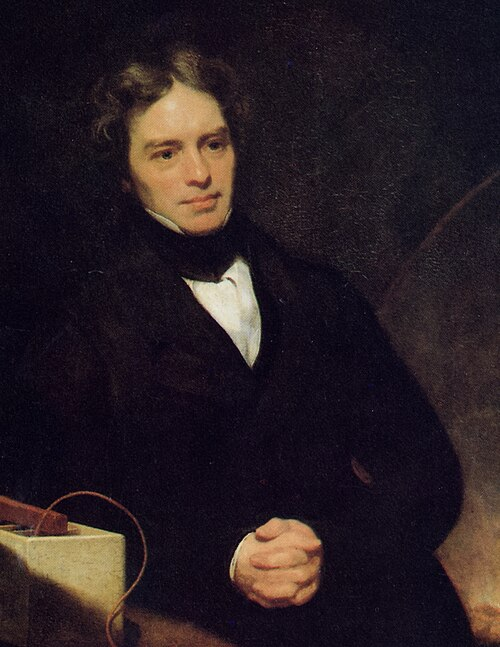
\includegraphics[width=\linewidth]{images/book3/faraday.jpg}
\end{minipage}\hfill
\begin{minipage}[t]{0.69\linewidth}
\vspace{0pt}
In 1834 stelde Michael Faraday, die de producten van elektrolyses mat met een
voltameter van eigen ontwerp, dat de massa van een stof die aan een elektrode ontstaat,
evenredig is met de doorgevoerde hoeveelheid elektriciteit, en
dat bij een gegeven hoeveelheid elektriciteit de massa's van verschillende stoffen
zich verhouden als hun chemische equivalenten. Hij bedacht de woorden
elektrode, anode, kathode, ion, anion en kation. De constante die zijn
naam draagt, maakt van die wetten $Q = nF\,\Delta\xi$. (Portret door Thomas Phillips,
1842, publiek domein, Wikimedia Commons.)
\end{minipage}
\end{history}

\section{Concentratiecellen}

\begin{definition}[Concentratiecel]\label{def:b2:cell-thermodynamics:concentration-cell}
Een \emph{concentratiecel}\index{concentratiecel} bestaat uit twee
halfcellen van hetzelfde koppel die alleen verschillen in de concentratie (of de
druk) van één deeltje.
\end{definition}

\begin{proposition}[Spanning van een concentratiecel]\label{prop:b2:cell-thermodynamics:concentration-cell}
Twee elektroden van een metaal M die in oplossingen van \ce{M^{n+}} dompelen met
concentraties $c_1 < c_2$, verbonden door een zoutbrug, geven een spanning
\[
  U = \frac{RT}{nF}\ln\frac{c_2}{c_1} ,
\]
waarbij de pluspool de meer geconcentreerde kant is. De cel werkt tot de
twee concentraties gelijk zijn.
\end{proposition}

\begin{proof}
Volgens de vergelijking van Nernst heeft elke elektrode $E_i = E^\circ + (RT/nF)\ln c_i$ (\omterm{def:b2:chemical-potential:ideal-mixture}{ideaal
verdunde oplossingen}); $E^\circ$ valt weg in het verschil. De reactie is
\ce{M^{n+}}(kant 2) $\to$ \ce{M^{n+}}(kant 1): metaal zet zich af aan de
geconcentreerde kant (kathode) en lost op aan de verdunde kant (anode), wat
de concentraties gelijkmaakt; $\Delta_r G = RT\ln(c_1/c_2) < 0$ tot ze
gelijk zijn.
\end{proof}

\begin{omfigure}
\begin{tikzpicture}[font=\small, >={Stealth}]
  \pic at (0,0) {beaker={0.7}{omDef!10}};
  \pic at (3.6,0) {beaker={0.7}{omDef!32}};
  \pic at (-0.3,0.25) {electrode={black!25}};
  \pic at (3.9,0.25) {electrode={black!25}};
  \pic at (0.35,0.55) {saltbridge={2.9}};
  \pic (m) at (1.8,4.3) {meter={V}};
  % common (black) terminal on the anode side, red (+) on the cathode side
  \fill[black] (1.4,4.03) circle (0.065); \fill[red!70!black] (2.2,4.03) circle (0.065);
  \draw[thick] (-0.15,2.65) |- (m-a);
  \draw[thick] (4.05,2.65) |- (m-b);
  \node[anchor=east] at (-0.95,1.0) {\ce{Ag}};
  \node[anchor=west] at (4.45,1.0) {\ce{Ag}};
  \node at (0.25,-0.35) {\ce{Ag+} \qty{0.010}{mol/L}};
  \node at (3.6,-0.35) {\ce{Ag+} \qty{0.10}{mol/L}};
  \node[anchor=east] at (-0.9,2.3) {$-$ anode};
  \node[anchor=west] at (4.6,2.3) {kathode $+$};
  \node[font=\scriptsize] at (-0.1,-0.8) {\ce{Ag -> Ag+ + e-}};
  \node[font=\scriptsize] at (3.7,-0.8) {\ce{Ag+ + e- -> Ag}};
  \node[font=\scriptsize] at (1.8,5.05) {$U = \qty{59}{mV}$};
\end{tikzpicture}

{\small Een \omterm{def:b2:cell-thermodynamics:concentration-cell}{concentratiecel} met zilver bij \qty{25}{\degreeCelsius}. De verdunde kant is
de anode: daar lost zilver op, en het zet zich af aan de geconcentreerde kant,
tot de twee concentraties gelijk zijn. $U = 0.0592\log(0.10/0.010) =
\qty{59}{mV}$.}
\end{omfigure}

Hetzelfde principe meet concentraties. Een glaselektrode, waarvan het dunne
membraan een referentieoplossing van het monster scheidt, ontwikkelt een
membraanpotentiaal van $(RT/F)\ln 10 = \qty{59}{mV}$ per eenheid pH-verschil bij
\qty{25}{\degreeCelsius}: de pH-meter van het deel van jaar~1 is een \omterm{def:b2:cell-thermodynamics:concentration-cell}{concentratiecel}
voor \ce{H+}. Over het membraan van een levende cel creëren de ongelijke concentraties
van \ce{K+} op dezelfde manier een potentiaal van enkele tientallen millivolt.

\section{Oefeningen}

\begin{exercise}[$\star$]\label{exo:b2:cell-thermodynamics:1}
Bereken uit $\Delta_f G^\circ(\ce{H2O}, \text{l}) = \qty{-237.14}{kJ/mol}$ de
standaardspanning van de waterstof-zuurstofcel.
\end{exercise}

\begin{exercise}[$\star$]\label{exo:b2:cell-thermodynamics:2}
Een batterij heeft een capaciteit van \qty{1.0}{A.h}. Bereken de lading die ze bevat, in coulomb,
en de massa zink die aan haar anode verbruikt wordt (\ce{Zn -> Zn^2+ + 2e-}) wanneer ze
volledig ontladen is.
\end{exercise}

\begin{exercise}[$\star$]\label{exo:b2:cell-thermodynamics:3}
Een daniellcel levert \qty{1.10}{V} zonder stroom. Bereken $\Delta_r G$ voor één
mol zink en de maximale elektrische arbeid voor \qty{10.0}{g} zink.
\end{exercise}

\begin{exercise}[$\star$]\label{exo:b2:cell-thermodynamics:4}
Twee koperelektroden dompelen in koper(II)sulfaatoplossingen van \qty{1.0e-3}{mol/L}
en \qty{0.10}{mol/L}. Bereken de spanning bij \qty{25}{\degreeCelsius} en benoem de
polen.
\end{exercise}

\begin{exercise}[$\star\star$]\label{exo:b2:cell-thermodynamics:5}
Een cel ($n = 2$) heeft $E^\circ = \qty{1.015}{V}$ en $dE^\circ/dT = \qty{-4.0e-4}{V/K}$
bij \qty{298}{K} (gegevens voor de oefening). Bereken $\Delta_r G^\circ$, $\Delta_r S^\circ$ en
$\Delta_r H^\circ$.
\end{exercise}

\begin{exercise}[$\star\star$]\label{exo:b2:cell-thermodynamics:6}
De cel van \cref{exo:b2:cell-thermodynamics:5} ontlaadt één mol reactie
(a) reversibel; (b) bij \qty{0.90}{V}. Bereken in elk geval de elektrische arbeid en
de warmte die met de omgeving wordt uitgewisseld.
\end{exercise}

\begin{exercise}[$\star\star$]\label{exo:b2:cell-thermodynamics:7}
Bereken $E^\circ(\ce{Fe^3+}/\ce{Fe})$ uit de vormingsgibbsenergieën
(\ce{Fe^2+} \qty{-78.90}{kJ/mol}, \ce{Fe^3+} \qty{-4.7}{kJ/mol}) en controleer dat ze
gelijk is aan $(E_1^\circ + 2E_2^\circ)/3$.
\end{exercise}

\begin{exercise}[$\star\star$]\label{exo:b2:cell-thermodynamics:8}
Bereken de standaardpotentiaal van het koppel \ce{AgCl}/\ce{Ag}, en daarna de
potentiaal van een zilverchloride-elektrode die in kaliumchloride van \qty{0.10}{mol/L}
dompelt.
\end{exercise}

\begin{exercise}[$\star\star$]\label{exo:b2:cell-thermodynamics:9}
Zink-luchtcellen gebruiken \ce{2Zn + O2 -> 2ZnO} ($\Delta_f G^\circ(\ce{ZnO}) =
\qty{-318.30}{kJ/mol}$). Bereken de standaardspanning en de maximale elektrische
energie, in \unit{kW.h}, per kilogram zink.
\end{exercise}

\begin{exercise}[$\star\star\star$]\label{exo:b2:cell-thermodynamics:10}
Een directe-methanolbrandstofcel werkt met \ce{CH3OH(l) + 3/2O2 -> CO2 + 2H2O(l)}. Bereken uit
$\Delta_f H^\circ$ (\unit{kJ/mol}): \ce{CH3OH(l)} $-239$, \ce{CO2} $-393.51$,
\ce{H2O(l)} $-285.83$; en $S^\circ$ (\unit{J/(K.mol)}): \ce{CH3OH(l)} 127.2,
\ce{CO2} 213.8, \ce{H2O(l)} 69.95, \ce{O2} 205.15 de waarden van $n$ en $E^\circ$ en het
maximale rendement.
\end{exercise}

\begin{exercise}[$\star\star\star$]\label{exo:b2:cell-thermodynamics:11}
Een cel ($n = 2$) heeft $E = \qty{0.500}{V}$ en $dE/dT = \qty{+3.0e-4}{V/K}$ bij
\qty{298}{K} (gegevens voor de oefening). Toon aan dat ze, reversibel werkend, meer
elektrische arbeid levert dan $-\Delta_r H$, en leg uit waar de extra energie vandaan komt.
\end{exercise}

\begin{exercise}[$\star\star\star$]\label{exo:b2:cell-thermodynamics:12}
Twee waterstofelektroden (\qty{1}{bar} \ce{H2}) dompelen in een referentieoplossing met
pH 7.00 en in een monster. De spanning is \qty{0.177}{V} bij \qty{25}{\degreeCelsius},
met de referentie als pluspool. Bepaal de pH van het monster, en leg uit
waarom het resultaat van geen enkele standaardpotentiaal afhangt.
\end{exercise}

\section{Probleem: de brandstofcelbus}

\begin{problem}[{Weekendprobleem --- de standaardspanning van de
waterstof-zuurstofcel uit gibbsenergieën, haar temperatuurcoëfficiënt, het
rendement en de warmte van een echte stapel, en de energie in een tank waterstof}]
\label{pb:b2:cell-thermodynamics:1}
Een brandstofcelstapel heeft 400 cellen in serie, elk met een protonwisselend
membraan (zuur elektrolyt). Gegevens bij \qty{298.15}{K} (CODATA, JANAF):
$\Delta_f H^\circ(\ce{H2O}, \text{l}) = \qty{-285.83}{kJ/mol}$, $\Delta_f
G^\circ(\ce{H2O}, \text{l}) = \qty{-237.14}{kJ/mol}$, $\Delta_f G^\circ(\ce{H2O},
\text{g}) = \qty{-228.58}{kJ/mol}$; $S^\circ$ (\unit{J/(K.mol)}): \ce{H2O(l)} 69.95,
\ce{H2} 130.68, \ce{O2} 205.15. $F = \qty{96485}{C/mol}$; $M(\ce{H2}) =
\qty{2.016}{g/mol}$.
% ledger: dfh:H2O-l, janafG:H2O_l.298, janafG:H2O.298, s0:H2O_l, s0:H2_g, s0:O2_g, const:F, aw:H

\medskip
\noindent\textbf{Deel I --- De standaardspanning.}
\begin{enumerate}
  \item Schrijf de halfreacties aan de anode en aan de kathode op, en de
        celreactie.
  \item Hoeveel elektronen worden er per molecuul waterstof uitgewisseld?
  \item Bereken $E^\circ$ wanneer het water vloeibaar gevormd wordt.
  \item Bereken haar wanneer het water als damp vertrekt.
  \item Verklaar het verschil met de verdampingsgibbsenergie van water.
  \item Bereken $\Delta_r H^\circ$ en het maximale rendement bij \qty{298}{K}.
\end{enumerate}

\medskip
\noindent\textbf{Deel II --- Temperatuur.}
\begin{enumerate}[resume]
  \item Bereken $\Delta_r S^\circ$ voor vloeibaar water.
  \item Leid $dE^\circ/dT$ af.
  \item Schat $E^\circ$ bij \qty{80}{\degreeCelsius}, de werktemperatuur van de
        stapel.
  \item Vergelijk je methode met de JANAF-waarde bij \qty{400}{K}, $\Delta_f
        G^\circ(\ce{H2O}, \text{l}) = \qty{-221.01}{kJ/mol}$.
  \item Welke warmte wisselt de reversibele cel per mol waterstof uit bij
        \qty{298}{K}? Wordt ze opgenomen of afgestaan?
  \item Schat het maximale rendement bij \qty{80}{\degreeCelsius}.
\end{enumerate}

\medskip
\noindent\textbf{Deel III --- De echte stapel bij \qty{0.70}{V} per cel.}
\begin{enumerate}[resume]
  \item Bereken de elektrische arbeid per mol waterstof.
  \item Bereken het rendement betrokken op $\Delta_r H^\circ$ en op $\Delta_r G^\circ$.
  \item Bereken de warmte die per mol waterstof vrijkomt.
  \item Hoeveel daarvan is onvermijdelijk, en hoeveel is te wijten aan de stroom?
  \item De stapel levert \qty{300}{A}. Bereken het waterstofverbruik van één
        cel, en daarna van de stapel, in mol en gram per seconde.
  \item Bereken het elektrisch vermogen van de stapel.
  \item Bereken het warmtevermogen dat het koelcircuit moet afvoeren.
\end{enumerate}

\medskip
\noindent\textbf{Deel IV --- De tank.}
\begin{enumerate}[resume]
  \item Welke hoeveelheid waterstof zit er in \qty{5.0}{kg}?
  \item Welke lading gaat er door de cellen, opgeteld over alle cellen, wanneer
        deze waterstof geoxideerd wordt?
  \item Bereken de elektrische energie die de stapel levert, met elke cel bij
        \qty{0.70}{V}.
  \item Reken haar om naar kilowattuur.
  \item Hoelang kan de stapel zijn vermogen van vraag 18 leveren?
  \item Geef de elektrische energie die \qty{5.0}{kg} waterstof levert bij
        \qty{0.70}{V} per cel.
\end{enumerate}
\end{problem}
